% ED26-BM-RAT2021-1-3, exact Schurz2021 chapter, printed101--114.
\chapter{Evolution of Rationality}
\label{sec:p19-rationality-1-3}

Schurz's 2021 chapter argues for an interaction between specialized cognitive
mechanisms and general learning and reasoning. Its evolutionary account has
three dimensions---biological inheritance, cultural transmission and
individual acquisition---rather than one story about a genetically fixed
reasoning organ. The proposed account also separates cognitive success from
other effects on survival, well-being and cooperation. It is not a deduction
that every present response is accurate, optimal, or normatively justified
\cite[pp.~101--113]{Schurz2021EvolutionRationality}.

This treatment retains the source's actual social, linguistic, causal and
inferential examples, its competing explanations, both figures and all nine
notes. The additional empirical corpus is bounded to the actual main reports
of Onishi--Baillargeon's infant task and Herrmann and colleagues' comparative
battery. Other cited studies and historical reconstructions retain their
source-reported standing when their task-level or historical records are not
qualified here. Such standing is different from an independently established
effect or an audited cross-cultural generalization.

\section{The criterion of rationality is not an evolutionary observation}
\label{sec:p19-r13-criteria}

\begin{hbdefinition}{def:p19-r13-criteria}{The source's theoretical and practical criteria}
Theoretical rationality concerns acquiring predictively, causally or
explanatorily useful information about the world. Schurz adopts cognitive
success as its evaluation criterion. In the cited Schurz--Hertwig account,
success combines \emph{validity}, the proportion of a method's rendered
inferences that are correct, and \emph{applicability}, the proportion of
problems of the specified type on which the method renders an inference.
Here validity is an empirical correctness proportion, not the logical
notion of truth preservation in every model.

Practical rationality concerns action in the interests of human beings.
The chapter adopts two minimal evaluative goals: advancing the acting
person's interests and promoting cooperation among interaction partners,
possibly including nonhuman beings. These are stated commitments, not
conclusions obtained solely from facts about reproductive success.
\end{hbdefinition}

The source opens with science and technology increasing human power and
religious belief increasing happiness. Whether either thereby counts as
rational depends on the chosen evaluative dimension and on the relevant
values. Its Humean is--ought point and note~1 direct the reader to a separate
logical treatment; no unrestricted theorem forbidding even normative
tautologies from factual premises is asserted here. Likewise, a fitness
advantage is not automatically truth, welfare, justice or sound inference.

\begin{hblemma}{thm:p19-r13-success}{proved=annex:p19.r13.success}{What the product measures on a finite task record}
For a fixed record of \(N>0\) equally weighted problems, let a method answer
\(a>0\) problems correctly on \(c\) of them. With correctness validity
\(v=c/a\) and applicability \(u=a/N\), the product \(vu=c/N\)
is the proportion of all problems receiving a correct answer. For \(a=0\),
the corresponding total correct-answer proportion is zero; validity itself
is undefined unless a separate convention is adopted. This identity does
not weight unequal error costs, resource expenditure or different problem
frequencies, and does not show that evolution optimizes this metric.
\end{hblemma}

The source's generalized placebo discussion concerns a possible noncognitive
benefit of beliefs in protective supernatural agents. Note~2 names religious
variation, including China, and connects the proposal to positive-illusion
literature. The chapter supplies no controlled intervention, representative
population or effect estimate establishing a universal causal benefit of
religious belief. It is retained as an evolutionary functional hypothesis
and a contrast between cognitive and noncognitive targets, not a health
recommendation or an accepted population effect.

\section{Three channels of cognitive change}
\label{sec:p19-r13-channels}

\begin{hbdefinition}{def:p19-r13-channels}{Biological, cultural and individual processes}
Biological evolution transmits genetic information through reproduction,
with the chapter also noting epigenetic discussions. Cultural evolution,
in the source's broad sense, transmits acquired information across
generations through social learning. Individual learning changes a person's
expectations or behavior through experience within that person's lifetime.
Reproduction, variation and selection characterize the source's generalized
Darwinian account of the first two channels; applying that account to the
third requires specifying which components actually occur.
\end{hbdefinition}

The technological example runs from Stone Age tools to automated production
and electronic intelligence. The argument is that acquired solutions can
be transmitted, modified and differentially retained without being copied
as genes; science and law supply further cultural examples. Note~4 names
early cultural-evolution models and later developments. Note~5 records the
controversy about Dawkins's ``meme'' terminology. Neither an analogy with
genes nor that name identifies a single experimentally established cultural
replicator or a uniform inheritance mechanism.

The individual channel has two importantly different examples. Operant
trial-and-error learning varies behavior and changes its frequency with
positive or negative feedback. Its within-lifetime analogue of transmission
is retention, unless the acquired behavior also enters social transmission.
Classical conditioning is illustrated by a bell predicting food and
salivation. The source instead characterizes association learning as directly
environment-guided induction, not blind spontaneous variation followed by
selection. Its use of ``Lamarckian'' is this comparison of learning modes,
not a claim that every learned association is genetically inherited.

The chapter's broad claims about conditioning across animal groups and its
Hebbian/neural account are attributed to its cited literature. The source
provides no common conditioning protocol, species sampling frame or
neurophysiological dataset from which those universal claims can be
recomputed. Note~3 also warns that the cited Jablonka--Lamb account uses
four evolutionary dimensions; it is not silently collapsed into the chapter's
three-channel terminology.

Genetic anchoring does not mean a unique response under every input. Note~9
explicitly allows one fixed mechanism to produce different behavior in
different environments. Conversely, correcting a judgment or adopting a
new explanation need not erase a perceptual appearance. The chapter's
plasticity argument is that acquired capacities can correct or override
some outputs, not a proof that every innate mechanism can always be removed.

\begin{figure}[htbp]
\centering
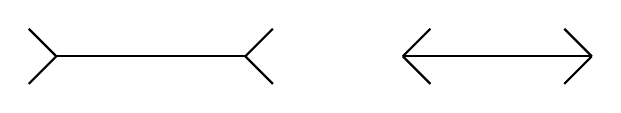
\begin{tikzpicture}[x=1cm,y=1cm]
\draw[thick] (0,0)--(2.4,0);
\draw[thick] (0,0)--(-.35,.35) (0,0)--(-.35,-.35);
\draw[thick] (2.4,0)--(2.75,.35) (2.4,0)--(2.75,-.35);
\draw[thick] (4.4,0)--(6.8,0);
\draw[thick] (4.4,0)--(4.75,.35) (4.4,0)--(4.75,-.35);
\draw[thick] (6.8,0)--(6.45,.35) (6.8,0)--(6.45,-.35);
\end{tikzpicture}
\caption{The source's Figure~1.3.1 comparison, reconstructed with equal
horizontal lengths: its left configuration can appear longer. The chapter
uses the M\"uller--Lyer illusion to distinguish a misleading appearance from
knowledge that the lengths are equal; its perspective account is one
attributed explanation, not a new perceptual experiment.}
\label{fig:p19-r13-muller-lyer}
\end{figure}

Kant's claim about necessarily Euclidean, three-dimensional perceived space
provides the other illustration. Mathematical education permits reasoning
about non-Euclidean and higher-dimensional spaces. Conceptualizing those
spaces is different from demonstrating a changed visual mechanism. The
illusion and geometry examples therefore support a distinction between
representation, judgment and reflective correction rather than a universal
genetic-determinism claim.

\section{Social cognition, language and cooperation}
\label{sec:p19-r13-social}

The source contrasts trained nonhuman symbolic signaling with human
productive syntax and proposes sociolinguistic coevolution: communication,
joint intentions, cooperation and language learning reinforce one another.
Large-prey hunting supplies its coordination example. The chapter's proposed
one-to-two-million-year genealogy is a historical evolutionary hypothesis,
not a time estimate derived from a measured sample of present infants.

Its account distinguishes cultural invention from subsequent genetic
assimilation through changed selection pressures, the Baldwin-effect
comparison. It cites Thompson--Kirby--Smith's 2016 simulations and
mathematical work against the inference that an apparently widespread
grammar necessarily requires strong innate grammatical determination.
The model's amplification claim depends on its learning and transmission
rules. No participant sample or observed historical allele trajectory is
supplied by that model attribution. The survey does not provide the full
model's equations, parameter domain or proof; its result remains a bounded
import, not a theorem about every possible learner or culture.

\subsection{Equilibrium, emergence and practical cooperation}

The chapter compares Hawk--Dove, coordination and prisoner's-dilemma
interactions. In the first, mixed behavior can be stable; in coordination
games several pure equilibria can coexist; in a one-shot prisoner's dilemma
individual defection incentives obstruct mutual cooperation. Strategy space,
payoffs, matching, repetition and dynamics determine what each statement
means. The presence of a cooperative equilibrium and its emergence from
every initial population are distinct properties.

\begin{hbexample}{def:p19-r13-stag-game}{A stated stag-hunt comparison}
Use the symmetric payoff to the row player
\[
\begin{array}{c|cc}
 &\text{Stag}&\text{Hare}\\\hline
\text{Stag}&5&0\\
\text{Hare}&3&3
\end{array}
\]
This is an illustrative model, not the original book's unspecified numerical
game. A cooperative resident earns five against another cooperative resident,
whereas a rare hare mutant earns three. Cooperation can be locally resistant
to invasion while a population with too few stag hunters favors hare.
\end{hbexample}

\begin{hblemma}{thm:p19-r13-stability}{proved=annex:p19.r13.stability}{Local evolutionary stability does not imply a global attraction basin}
In the stated game, a population with fraction \(x\) stag earns row payoffs
\(5x\) for stag and \(3\) for hare. Under the two-strategy replicator
equation \(\dot x=x(1-x)(5x-3)\), the dividing frequency is \(3/5\).
The pure stag strategy is evolutionarily stable against sufficiently rare
hare invasion, but initial \(x<3/5\) moves toward hare. Thus breakdown
after a sufficiently large change does not refute local evolutionary
stability. This repairs the source's conflation without asserting the
illustrative payoffs were its empirical inputs.
\end{hblemma}

The source's tit-for-tat example begins cooperatively and then copies the
partner's preceding action, rewarding cooperation and retaliating against
defection. Its universal-optimality reading is not adopted. The cited
Lorberbaum result has a specified repeated-game strategy and invasion
setting; it is not a universal theorem for every population structure,
noise model or sanction system. The source lists five further mechanisms:
regrouping/group selection, communication and correlated pairing,
institutional sanctions, cheater detection, and religious stabilization of
altruism. These are different hypotheses or interventions, not mutually
interchangeable demonstrations of cooperation.

Note~6 makes ``egoistic'' and ``cooperative'' evolutionary payoff roles,
not automatic diagnoses of psychological motivation. The historical contrast
between reputation in small groups and institutions in larger agricultural
communities supplies the chapter's explanatory narrative. Its references
to Hammurabi, hunter--gatherer sharing and proto-state sanctions do not
constitute a systematic dataset establishing that every known society
followed one path. Hammurabi is used as a codification example, not asserted
to be the earliest surviving juridical document.

\subsection{Mindreading mechanisms and a task-specific infant record}

The source's developmental sequence includes shared attention around nine
months, later pointing and language learning, and the ability to represent
another person's intentions and beliefs. It contrasts specialized
theory-of-mind accounts with simulation accounts that reuse machinery for
one's own attitudes to simulate another's. Evolutionary economy is an
argument for considering reuse, not evidence that fewer postulated modules
must be the actual mechanism.

\begin{hbdefinition}{def:p19-r13-onishi}{The selected 2005 nonverbal false-belief task}
Onishi and Baillargeon analyzed 56 healthy-term infants, 27 female and
29 male, mean age 15 months 7 days, range 14 months 27 days to
15 months 18 days. Another 14 tested infants were excluded: inattention
four, condition-mean outliers beyond three standard deviations four,
fussiness two, parental interference two, and observer error two.
Seven were randomly assigned to each cell of a \(2\times2\times2\)
between-infant design: actor's believed location, true/false belief,
and reached-for location. After three familiarization trials and one
belief-induction trial, test looking duration assessed expectation violation.
The belief-location by reached-location interaction was
\(F(1,48)=31.24\), \(p<.0001\); the true- and false-belief subsets also
showed that interaction. These are looking-time effects, not percentages
passing a verbal question or measurements of inherited circuitry
\cite[pp.~255--258]{R13OnishiBaillargeon2005}.
\end{hbdefinition}

The four belief histories distinguish the actor's information from the
infant's actual-location information. The authors discuss simpler last-seen
and action-expectation accounts as well as their preferred rudimentary
belief interpretation. This design is not equivalent to Wimmer--Perner's
verbal false-belief task with preschoolers. The source's age contrast does
not by itself establish one age at which every component of belief
understanding appears. Supporting methods and population-level replication
require their separate records; no new reanalysis or confidence interval
for an infant population is claimed here.

The source adds conventional moral-stage and reciprocity claims, which it
attributes to Piaget, Kohlberg and social-exchange literature. These provide
its link to generalized rules and rule-breaker detection, not a dataset
showing all children reach a fixed universal stage on their sixth birthday.
Note~7 also withdraws a strong human-exclusive intentionality claim,
mentioning chimpanzee evidence and later anticipatory eye-movement tasks.
That correction is preserved: species differences in degree and task are
not absence of every relevant capacity in every nonhuman animal.

The argument for representations then goes beyond immediate stimuli:
different perceptual cues can indicate the same behaviorally relevant object
configuration, such as a bear in a cave. A representation can mediate several
cues and several actions rather than require a distinct direct association
for each pair. Schulz's efficiency account and the source's common-cause
abduction comparison are cited explanatory proposals; economy of a model
is not alone proof that a neural system implements it.

\section{Technological control and causal models}
\label{sec:p19-r13-causal}

Sociotechnical coevolution concerns manipulating the environment as well as
predicting it: fire, stone tools, weaving, weapons and agriculture are the
chapter's examples. It distinguishes an observed association from a model
of how an intervention changes an outcome. Its three explanatory candidates
for correlated events are forward causation, reverse causation and common
causation. In a specified acyclic causal model these illustrate why an
association does not identify an intervention; they are not asserted to
exhaust every selected, cyclic or mismeasured observational record solely
from a bare Markov slogan. The actual equation-replacement interface is
\cref{def:p16-finite-scm}.

\begin{hbdefinition}{def:p19-r13-herrmann}{The selected comparative battery}
Herrmann and colleagues tested 105 German children aged 2.5 years
(\(\pm2\) months), 106 sanctuary chimpanzees aged 3--21 years,
and 32 care-center orangutans aged 3--10 years. Six scales organized
16 tasks: space, quantities and causality; social learning, communication
and theory of mind. Human experimenters administered each individual's
3--5-hour battery over several days. Table~2 reports mean physical-domain
correct proportions \(.68,.68,.59\), and social-domain proportions
\(.74,.36,.33\), in that species order. Children and chimpanzees had no
detected overall physical-domain difference; children exceeded both ape
groups socially (reported post-hoc \(p<.001\)). Physical tasks had different
chance baselines; children did better on three causal-judgment tasks while
chimpanzees did better on active stick use. The comparison was not an
equivalence test or randomized genetic intervention
\cite[pp.~1360--1366, Tables~1--2]{R13HerrmannEtAl2007}.
\end{hbdefinition}

The study discusses human-constructed tasks, experimenter species,
temperament and alternative accounts involving hidden causes. It supports
a task-pattern comparison, not a universal ``cognitive age'' for an ape or
proof of a uniquely social genetic module. The chapter's approximate
three-year comparison is kept distinct from the actual 2.5-year cohort.
Its links among pretend play, counterfactual thought and causal modeling
remain proposed mechanisms or separately cited developmental findings.

The historical intentional/physical distinction connects people interpreting
actions through goals with contact-based explanations of inanimate motion.
The source links animation of weather or celestial motion to religious
explanation, and contrasts Leibniz's intentional interpretation with Hume's
epistemic challenge. This is an attributed genealogy, not evidence that
every early explanation or every culture used an identical mechanism.

The infant illustration compares a moving ball touching another before it
moves with the second ball moving without contact; it then contrasts a boy
approaching a girl with and without touch. The chapter reports longer gaze
at the noncontact inanimate event but no corresponding difference for people,
citing Leslie and Spelke--Phillips--Woodward. Its sample, exact age range,
duration distributions and uncertainty are not supplied in this survey.
The account therefore does not establish that all six-month-olds encode
adult intentions, or that gaze uniquely identifies the proposed module.
Magnets provide the later counterexample to an unchangeable contact-only
intuition: learning a reliable action-at-a-distance pattern need not
eliminate every earlier perceptual or explanatory disposition.

\section{Modularity, generality and changing environments}
\label{sec:p19-r13-modularity}

The source's modularist account treats a module as a purpose- or area-specific
process associated with an adaptive problem, not merely a region bearing
a convenient name. Its examples include shared attention, language
acquisition, spatial models, mindreading, physical/intentional causality,
conventional moral rules and cheater detection. The cited developmental
ages are source-attributed milestones with different tasks, not one common
longitudinal panel: physical/intentional causality around six months, shared
attention around nine months, language acquisition from eighteen months,
sensorimotor spatial models over zero--two years, mindreading around
four--five years, and conventional moral values around six years. These ages
have different measures and need not identify the same onset as a nonverbal
task. The adaptive-toolbox view adds a procedure--environment
fit and the possibility that less information or computation can sometimes
be more useful.

Generalist models instead seek processes usable across problems. The source
recalls logicist expectations, later probabilistic alternatives, and task
deviations from both. Its contemporary compromise does not deny specialized
abilities: it argues that unexpected environmental change also favors
learning and reasoning not fixed to one narrow problem. The human-hand
comparison contrasts flexible reuse with a Swiss-army-knife image. Even
some evolutionary-psychology accounts admit improvisational intelligence.
The source also invokes an approximately 200,000-year evolutionary timescale
against a module for every possible task. This is its cited plausibility
argument, not a proved upper bound on the number of cognitive mechanisms.
Naming all general capacities ``modules'' would obscure the disputed
specificity rather than settle it.

Purpose-specificity and domain-specificity are nonidentical dimensions.
The chapter argues that they often covary; it supplies no sample or
correlation estimate proving a universal relation. The actual heuristic
comparison in \cref{def:p19-r24-benchmark} requires a target, available
information, resource costs and an evaluation environment. The principle,
positive theory and prescription distinction in
\cref{def:p17-br-principle-theory,def:p17-br-three-rationalities}
likewise prevents fitting a response pattern from automatically proving
a recommended procedure.

\section{Induction, method selection and the conditional examples}
\label{sec:p19-r13-inference}

Association learning is the source's most general example of inductive
projection. Its usefulness under varied tasks does not solve Hume's
justification problem. The chapter states that observations do not
deductively demonstrate the future's uniformity, and that appealing to
past inductive success would use the contested procedure. It contrasts
this with Reichenbach's best-available-method approach and Schurz's
meta-induction proposal.

The described meta-inductivist observes the performance records of accessible
methods and periodically updates a success-dependent weighted combination.
The source cites formal optimality and social-spread work; it does not
provide a complete update rule, loss convention, comparator class or horizon
in this chapter. Its all-worlds wording is therefore a source-cited relative
guarantee for a defined prediction/decision setting, not immediate
perfection, an inaccessible oracle comparison, or biological evidence that
each person uses that method. Nor is it a guarantee of transfer to hidden
feedback, an altered payoff scale or unlimited unobserved competitors.

\begin{hblemma}{thm:p19-r13-horizon}{proved=annex:p19.r13.horizon}{Long-run comparison permits an individual error}
A comparator claim \((L_T-L_T^*)/T\to0\) about cumulative losses is
compatible with a nonzero error at a finite time: the loss records
\(L_T=1\), \(L_T^*=0\) for all \(T\geq1\) have normalized gap
\(1/T\to0\). This separates an asymptotic statement's logical strength
from universal correctness on every individual problem; it is not asserted
as the full theorem of the source's meta-inductive strategy.
\end{hblemma}

The chapter distinguishes evolutionary priority from justificatory priority:
learning may precede explicit logic in phylogeny, while justifying a learning
argument still uses logical relations. Neither priority makes a psychological
implementation of a formal calculus a proved biological adaptation.
Its report of modus-ponens competence around age six, contrasted with adult
modus-tollens difficulty, is a developmental-literature attribution, not a
task-independent age-of-mastery estimate without the original records.

Its abstract four-card example uses A, B, 1 and 2 to test the rule that
A must have 1 on the other side. With a letter on one face and a number
on the other, complete falsification testing requires A and 2. B and 1
cannot expose a violation regardless of their hidden faces. This is the
renamed benchmark proved in \cref{thm:p19-r23-cards}. Choosing a card
to investigate a rule is not directly executing modus ponens or modus
tollens under an already accepted rule. A literal empirical frequency
of rule execution cannot be inferred just from a selection frequency.

The source's social regulation concerns alcohol consumption and a minimum
age of sixteen, with two beverages and two ages exposed. The counterexample
checks are the alcohol drinker and the under-sixteen person; named actors
do not change that benchmark. The source's 100/5/10/5 abstract-task
percentages and its universal-perfect social-task statement lack a recoverable
sample denominator and exact response-category definition in the chapter.
They are not adopted as new population estimates. The source Griggs--Cox
attribution concerns thematic facilitation; its task and full response tables
need their own qualified original record. The actual larger selection-task
database, with abstract/everyday/deontic denominators and limitations, is
already distinguished in \cref{sec:p19-r23-testing}.
The named adolescents and sixteen-year rule are the chapter's instantiation;
they are not asserted to be the unchanged administered materials of the
cited 1982 experiments.

The chapter favors the cheater-detection hypothesis and cites contrasts with
pragmatic deontic schemas and utility accounts, including its source-reported
claim that beneficial social exchange is important. Competing content,
familiarity, interpretation and goal effects do not vanish merely because
the hypothesis has an evolutionary explanation. The source combines that
specialization with a general probabilistic reading of uncertain ordinary
conditionals. The detailed belief-versus-frequency and conditional-query
distinctions are \cref{sec:p19-rationality-4-6}.

\begin{hblemma}{thm:p19-r13-probabilistic-mt}{proved=annex:p19.r13.probabilistic-mt}{High conditional probability does not license unrestricted probabilistic contraposition}
An arbitrarily high \(P(B\mid A)\) alone does not force high
\(P(A^c\mid B^c)\). For \(0<\epsilon<1\), put
\(P(A\cap B)=1-\epsilon\), \(P(A\cap B^c)=\epsilon\),
and both \(A^c\) cells zero. Then
\(P(B\mid A)=1-\epsilon\), but \(P(A^c\mid B^c)=0\).
Material modus tollens remains valid under its own true material-conditional
premise; these are different premise semantics, not a failure of logic.
\end{hblemma}

Thus the source's evolutionary reconciliation is a proposal about interaction:
specific social checks and broader uncertain-conditional procedures may both
be useful under different inputs and goals. The countermodel proves only
the stated probability distinction. It does not show that every participant
used conditional probability or that it uniquely explains an abstract-card
error. The actual suppression and mental-model records in Part XIX keep
the interpretation and mechanism questions distinct.

\section{The proposed architecture and its evidential standing}
\label{sec:p19-r13-architecture}

The source's conclusion gives consciousness a limited but substantial role.
Many specialized processes and some general inductive processes operate
without awareness. It rejects a purely epiphenomenal reporter view by
appealing to reflective correction, formal reasoning and institutionalized
scientific work. The road-crossing illustration contrasts rapid intuitive
estimation with slow explicit calculation, but supplies no timing experiment
or measured universal speed ratio. Scientific institutions protect some
deliberation from immediate action pressure; this is a proposed enabling
condition, not proof that reflective cognition is always superior or free
of simplification.

\begin{table}[htbp]
\centering\small
\begin{tabularx}{\textwidth}{@{}l X X@{}}
\toprule
Source level & Proposed capacity layer & Source consciousness/acquisition description \\
\midrule
Invertebrate base & Sensory and motor modules & Unconscious and innate \\
Vertebrate layer & Results of inductive conditioning & Unconscious and learned \\
Hominids/humans; primates questioned & Area-specific cognitive models/modules & Partly conscious and partly innate \\
Modern human upper layer & Universal mind/reason & Fully conscious and learned \\
\bottomrule
\end{tabularx}
\caption{All tiers and uncertainty in the source's Figure~1.3.2, represented
as a consultation table. The tiers coexist in the proposed layered account;
the animal labels are not disjoint sampled populations, and the diagram
is not a measured phylogenetic timeline or a verified partition of brain
systems. Its upper-layer wording describes the author's schematic ideal.}
\label{tab:p19-r13-architecture}
\end{table}

Euclidean geometry and perspective, formal logic and probability, relativity,
quantum theory, evolution and computing are the source's examples of cultural
achievements beyond an immediate heuristic response. The chapter's historical
names include Euclid, Leonardo, Minkowski, Aristotle, Boole, G\"odel,
Einstein, Bohr and Darwin. Its argument is for flexible general reasoning
supported by institutions and specialized representations. It is not proof
that all perceptual deception has disappeared, every intuitive error is
detectable in practice, or every modern individual's inference is optimal.

\section{Using the evolutionary account without an invalid transfer}

For consultation, distinguish an observed task effect, a model prediction,
a developmental claim, a proposed evolutionary function and an adopted
normative goal. A genetic disposition can be context-sensitive; a culturally
shared outcome can depend on learned transmission; individual success can
reflect experience rather than an independently evolved module. The present
phenotype does not identify a unique ancestral selection history. Cross-task,
cross-species and historical extrapolations require the evidence conditions
of \cref{def:p19-evidence-record}.

\begin{longtable}{@{}p{.21\linewidth}p{.33\linewidth}p{.38\linewidth}@{}}
\caption{The chapter's mechanisms and their different verification demands.}
\label{tab:p19-r13-evidence-boundaries}\\
\toprule Claim type & Source contribution & What does not follow \\
\midrule\endfirsthead
\caption[]{The chapter's mechanisms and their different verification demands (continued)}\\
\toprule Claim type & Source contribution & What does not follow \\
\midrule\endhead
\midrule\multicolumn{3}{r}{\emph{continued on next page}}\\
\endfoot
\endlastfoot
Normative criterion & Cognitive success and interest/cooperation goals are explicitly adopted. & Fitness history alone does not entail truth, welfare or an ought claim. \\
Evolutionary mechanism & Reproduction/variation/selection, cultural transmission, retention and associative induction are distinguished. & Their shared vocabulary does not establish one inheritance process or inevitable improvement. \\
Developmental observation & Verbal false-belief, looking-time, comparative battery and contact-causality examples have different measures. & A response or gaze effect does not uniquely identify an innate module or universal developmental age. \\
Strategic model & Payoffs and population dynamics explain local cooperation and invasion conditions. & A limited basin does not deny local ESS; no strategy is optimal under every unspecified repeated-game model. \\
Method comparison & Accessible success records motivate meta-inductive combination and changing-environment selection. & Relative long-run comparison is not per-trial perfection or evidence of actual ancestral implementation. \\
Reflective correction & Geometry, magnets and institutional science illustrate new representations and checking. & Correct judgment does not necessarily remove an illusion or make conscious thought invariably better. \\
\bottomrule\end{longtable}

The bibliography intake retains the source's complete reference identities
and version information, without claiming that every referenced book has
been acquired or assigning its whole contents to this treatment. The source's
historical and evolutionary proposals and the actual selected experiments
remain separately attributed. Their comparison can guide a testable account;
it does not substitute an adaptation label for evidence of its mechanism.
\nocite{Schurz2021EvolutionRationality,R13OnishiBaillargeon2005,R13HerrmannEtAl2007,R13Adams1975,R13Almor2003,R13Aunger2002,R13Axelrod2006,R13BarbeySloman2007,
R13BarkowCosmidesTooby1992,R13BarrettCosmidesTooby2007,R13Basalla1988,R13Bitterman2000,R13BlockFlanaganGuzeldere1996,R13BoydRicherson1985,R13Boyer1994,R13Brainerd1978,
R13BuchsbaumEtAl2012,R13CallTomasello2008,R13Campbell1960,R13CarruthersChamberlain2000,R13CavalliSforzaFeldman1973,R13CesaBianchiLugosi2006,R13ChengHolyoak1985,R13Chomsky1968,
R13Churchland1979,R13CosmidesBarrettTooby2010,R13CosmidesTooby1992,R13CosmidesTooby2015,R13Dawkins1987,R13DeliusJitsumoriSiemann2000,R13Dennett1995,R13Dennett2018,
R13DuchaineCosmidesTooby2001,R13Dunbar2000,R13Evans1982,R13Evans2002,R13EvansHandleyOver2003,R13Gehlen1977,R13GigerenzerSelten2001,R13GigerenzerToddABC1999,
R13GriggsCox1982,R13GurerkIrlenbuschRockenbach2006,R13Henrich2016,R13Heyes2012,R13HeyesFrith2012,R13Hume2004,R13Hume2006,R13InhelderPiaget1958,
R13JablonkaGinsburgDor2012,R13JablonkaLamb2005,R13Kahneman2011,KahnemanTversky1972Subjective,R13Kohlberg1984,R13KrupenyeEtAl2016,R13Leslie1982,R13Leslie1987,
R13Lewis1973Causation,R13Lorberbaum1994,R13ManktelowOver1991,R13Mesoudi2011,R13Millikan2002,R13NicholsStich2003,R13OaksfordChater1991,R13Over2003,
R13Papineau2003,R13Pearl2009,R13PfeiferKleiter2010,R13Piaget1932,R13RafetsederEtAl2013,R13Reichenbach1938,R13Rock1984,R13Rojas1996,
R13Schulz2011,R13Schulz2018,R13Schurz1997,R13Schurz2001,R13Schurz2008,R13Schurz2011,R13Schurz2012,R13Schurz2016,
R13Schurz2019,R13SchurzGebharter2016,R13SchurzHertwig2019,R13SchurzThorn2012,R13SchurzThorn2016,R13Skyrms2004,R13Skyrms2010,R13Sober1993,
R13SoberWilson1998,R13SpelkePhillipsWoodward1995,R13SpirtesGlymourScheines2000,R13Sterelny2012,R13Taylor1989,R13ThompsonKirbySmith2016,R13ThornSchurz2019,R13Thorndike1911,
R13ToddGigerenzerABC2012,R13Tomasello1999,R13ToobyCosmides1992,R13Topitsch1979,R13Wason1966,R13Weibull1995,R13Wenegrat1990,R13Wilson2002,
R13WimmerPerner1983,R13Woodward2003}
\index{evolution of rationality}\index{cognitive success}\index{cultural evolution}
\index{biological evolution!reasoning}\index{mindreading!task evidence}
\index{modularity!domain and purpose}\index{meta-induction!guarantee boundary}
